\documentclass[twocolumn]{aastex62}
\newcommand{\vdag}{(v)^\dagger}
\newcommand\aastex{AAS\TeX}
\newcommand\latex{La\TeX}
\usepackage{amsmath}
\usepackage{physics}
\usepackage{hyperref}
\usepackage{natbib}
\usepackage[T1]{fontenc}
\usepackage[english]{babel}
\usepackage[utf8]{inputenc}

\begin{document}

\title{Solving Eigenvalue Problems by Means of the Jacobi Algorithm}

\author{Håkon Tansem}

\author{Nils-Ole Stutzer}

\author{Bernhard Nornes Lotsberg}

\begin{abstract}
\end{abstract}

\section{Introduction} \label{sec:intro}
When solving problems in science and mathematics an ever recurring problem is to solve integrals. Integrals are found in all sorts of manners both directely and indirectely though e.g. differential equations. In this paper we will consider ways of solving an example of a six dimensional integral in several different ways. We will consider a brute force Gauss-Legendre quadrature, an improved Gauss-Laguerre quadrature, a brute force monte carlo integration and a monte carlo integration with importance sampling. The integral to solve is an expectation value problem from quantum mechanics. The resulting integrals will be compared to the analytical solution and the run times of each mothod are compared, in order to find which method is most efficient.

In the theory section we present needed theory wich we discuss how to implement in the method section. The results are presented in the results section and discussed in the discussion section.

\section{Theory} \label{sec:theory}
\subsection{The integral}
Before stating the needed integration methods we used we present the integral to integrate.

First we assume that the wave function of two electrons can be modelled like a the single-particle wave function of an electron in the hydrogen atom. The wave function of the $i$th electon in the 1 $s$ state is given in terms of
\begin{align}
	\vec{r}_i = x_i \hat{e}_x + y_i\hat{e}_y + z_i\hat{e}_z
\end{align} 
the dimensionless posission, where $\hat{e}_i$ are orthonormal unit vectors, so that the wave function
\begin{align}
	\psi_{1,s}(\vec{r}_i) = e^{-\alpha r_i}.
\end{align}
The distance $r_i = \sqrt{x_i^2 + y_i^2 + z_i^2}$ and we let the parameter $\alpha = 2$ corresponding to the charge of a helium $Z = 2$. Then the ansats for the wave function for two electrons is given by the product of the two 1 $s$ wave functions 
\begin{align}
	\Psi(\vec{r}_1, \vec{r}_2) = e^{-\alpha(r_1 + r_2)}.
\end{align}
We now want to find the expectation value of the correlation energy between electrons which repel each other by means of the Coulomb interaction as 
\begin{align}
\label{eq:cartint}
\langle \frac{
1}{\vec{r}_1 - \vec{r}_2}\rangle = \int^\infty_{-\infty} d\vec{r}_1d\vec{r}_2 e^{-2\alpha(r_1 + r_2)}\frac{1}{|\vec{r}_1 - \vec{r}_2|}.
\end{align}
This integral has an analytical solution $5\pi^2/16^2$, which we can later compare with.
\subsection{Brute force Gauss-Legendre quadrature}


\section{Method} \label{sec:method}
\subsection{Classical Wave - The Buckling Beam Problem}

\section{Results} \label{sec:results}
The results were produced running on a MacBook Pro (macOS Mojave 10.14.6) with
8gb RAM using a dual coreIntel Core i5-7360U $2.3$GHz CPU with four threads. The program was compiled
using openMP for the parallelization with the gcc compiler version (Homebrew GCC
$9.2.0\_1$) $9.2.0$.\\\\ When calculating the integral, the relative error was
calculated for the integral given by (\ref{eq:cartint}) using the brute force
method, as describred in section(REFERER TIL BRUTE FORCE QUAD SECTION). The
relative error was also calculated for the integral in spherical coordinates given by (REFERER TIL SFÆRISK
INTEGRAL) using the improved method, as described in section (REFERER TIL
IMPROVED GAUSSIAN QUAD SECTION). These results are shown in figure
\ref{fig:relerrquad}. In the figure a line is drawn when the relative error
surpasses $10^{-2}$ to illustrate when the method achieves three digit precision.\\
\begin{figure}[h]
	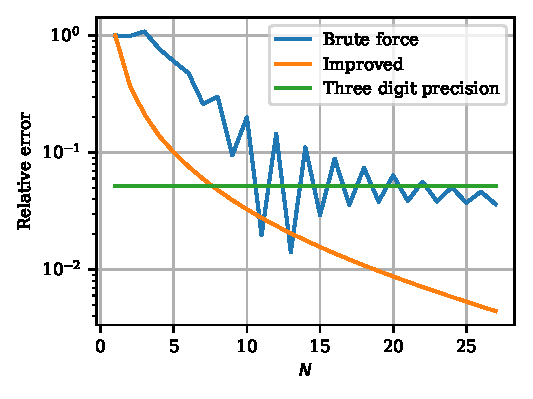
\includegraphics[scale=0.55]{{Figures/exercise_a_b}.pdf}
	\caption{Figure showing the relative error for the brute force gaussian quadrature and the improved gaussian quadrature methods described in section (REFERER TIL SEKSJON). A line is drawn when the relative error is $10^-2$ to illustrate when the integral reaches three digit precision.}
	\label{fig:relerrquad}
\end{figure}
The relative error was also compared for both the brute force Monte Carlo method
and the improved Monte Carlo method described in section (REFERER TIL BRUTE
FORCE) and (REFERER TIL IMPROVED) respectively. This is shown in figure
\ref{fig:rellerrcarlo}. For the same calculations using both Monte Carlo methods, the variance was also plotted.
This is result is illustrated in figure \ref{fig:variancecarlo}. 
\begin{figure}[h]
	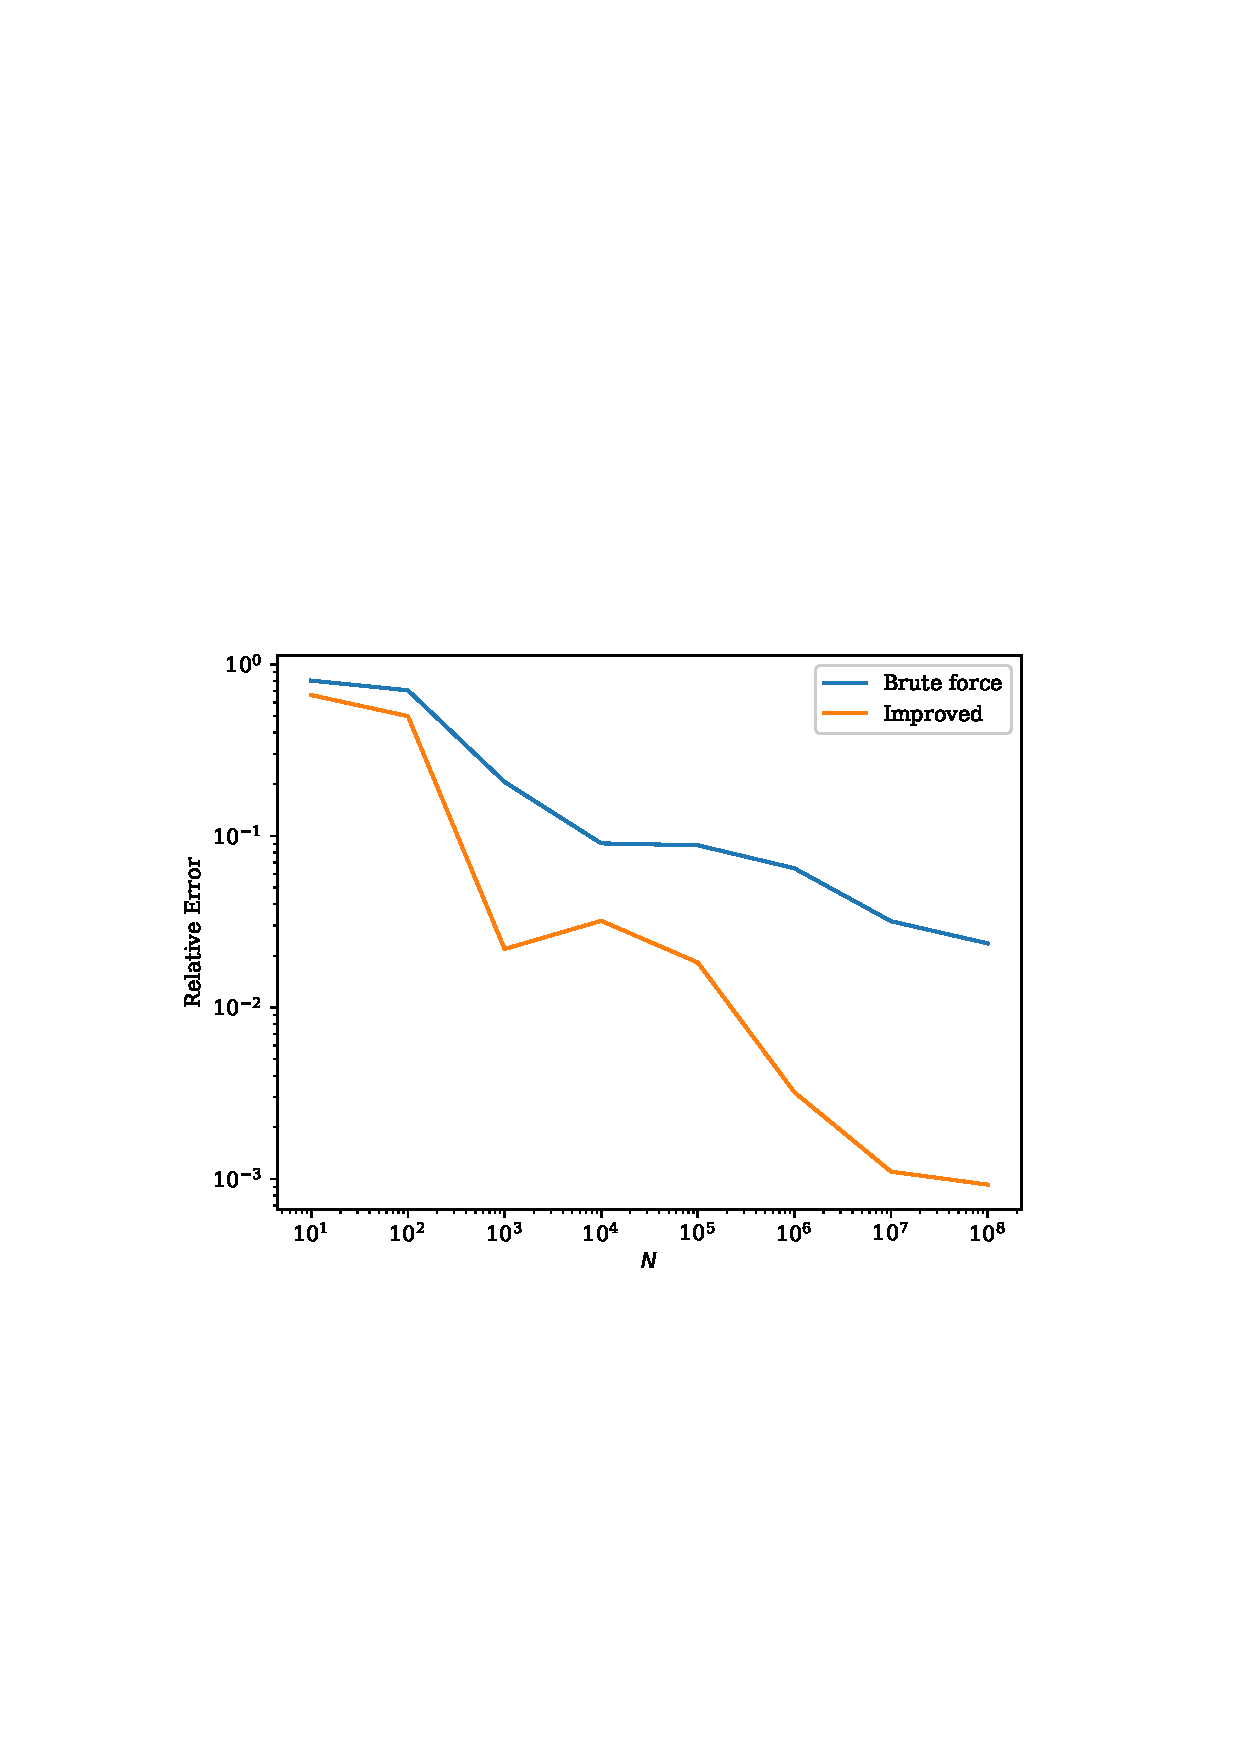
\includegraphics[scale=0.55]{{Figures/error_monte_carlo}.pdf}
	\caption{Figure showing the relative error for the brute force and the improved Monte Carlo methods described in section (REFERER TIL SEKSJON).}
	\label{fig:rellerrcarlo}
\end{figure}

\begin{figure}[h]
	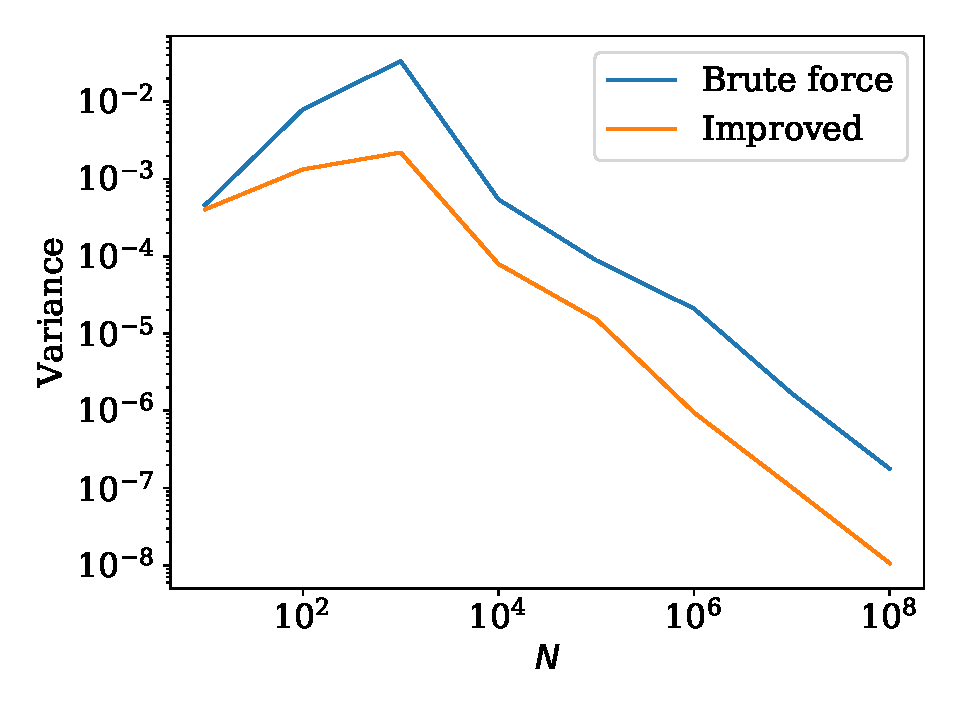
\includegraphics[scale=0.55]{{Figures/variance_monte_carlo}.pdf}
	\caption{Figure showing the variance for the brute force and the improved Monte Carlo methods as described in sections (REFERER TIL SEKSJONER) and respectively.}
	\label{fig:variancecarlo}
\end{figure}
The CPU time for both the brute force and the improved Monte Carlo methods was calculated using no
parallelization and parallelization with two threads. This is shown in figure
\ref{fig:CPUcarlo}. The three different compiler flags -O1, -O2 and -O3 was also
compared to study their impact on the CPU time, which is shown in figure
\ref{fig:CPUcarloflag}. This result was produced using parallelization with four
threads.
\begin{figure}[h]
	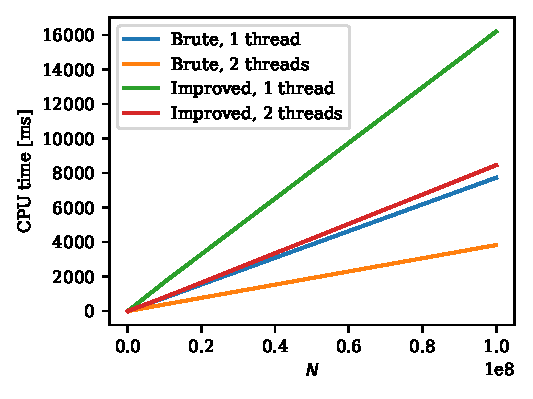
\includegraphics[scale=0.55]{{Figures/cpu_time_monte_carlo}.pdf}
	\caption{Figure showing the CPU time the brute force and the improved Monte Carlo methods described in section (REFERER TIL SEKSJON). For both methods the CPU time was compared both unparallelized and parallelized with two threads.}
	\label{fig:CPUcarlo}
\end{figure}

\begin{figure}[h]
	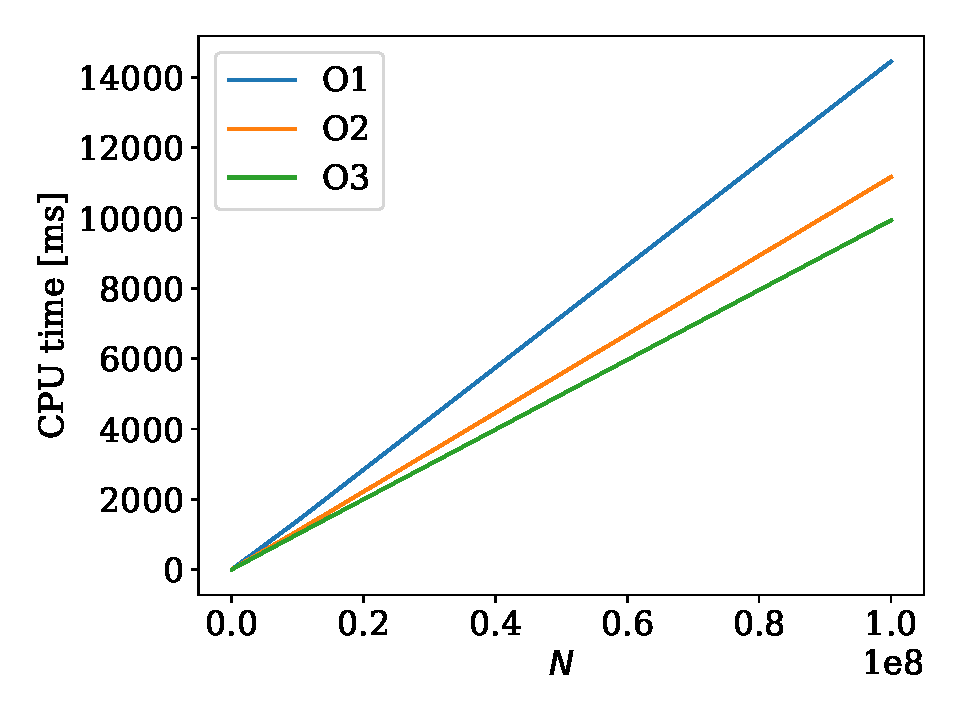
\includegraphics[scale=0.55]{{Figures/cpu_time_compilerflag}.pdf}
	\caption{Figure showing showing the CPU time for the improved Monte Carlo method, as described in section (REFERER TIL SEKSJON), using the different compiler flags -O1, -O2 and -O3. These results were produced using parallelization with four threads.}
	\label{fig:CPUcarloflag}
\end{figure}


\section{Discussion} \label{sec:discussion}
\section{Conclusion} \label{sec:conclusion}

%nocite{jensen:2019}
%\bibliographystyle{aasjournal}
%\bibliography{ref}

\end{document}

